\documentclass[12pt, a4paper, UTF8]{article}

\usepackage{ctex}
\usepackage{amsmath}
\usepackage{booktabs}
\usepackage{graphicx}
\usepackage{float}
\usepackage{caption}
\usepackage{setspace}
\setstretch{1.25}

\title{Project 4 实验报告\\Device Compact Modeling 参数提取}
\author{姓名：徐子翔 \quad 郦查德}
\date{\today}

\begin{document}

\maketitle

\section{实验目的}
本实验针对 65nm 平面 NMOS 的 BSIM4 模型进行手动参数提取。目标是通过参数调节使仿真曲线与目标数据对齐，并理解不同参数对应的物理意义与耦合关系。


\section{任务0：电容调整}

\subsection{原理分析}
本栅介质厚度参数定义为
\begin{equation}
	DTOX=TOXE-TOXP.
\end{equation}
其中 \(TOXE\) 为电学等效氧化层厚度，\(TOXP\) 为物理等效氧化层厚度。

外侧边缘电容 \(CF\) 的计算式为
\begin{equation}
	CF=\frac{2\cdot EPSROX\cdot\varepsilon_0}{\pi}\log\left(1+\frac{4.0\times10^{-7}}{TOXE}\right). \tag{BSIM4 (7.86)}
\end{equation}
此外，BSIM4 阈值模型中 \(NDEP\) 与 \(K1\) 的关系可写为：
\begin{equation}
	\Phi_s = 0.4 + \frac{k_B T}{q}\ln\left(\frac{NDEP}{n_i}\right) + PHIN. \tag{BSIM4 (2.11)}
\end{equation}
\begin{equation}
	\gamma_1 = \frac{\sqrt{2 q \varepsilon_{si} NDEP}}{C_{oxe}}. \tag{BSIM4 (2.15)}
\end{equation}
\begin{equation}
	K1 = \gamma_2 - 2K2\sqrt{\Phi_s - VBM}. \tag{BSIM4 (2.13)}
\end{equation}
其中 \(K1\) 在阈值电压公式（BSIM4 (2.10)）中直接控制体效应项，故会影响 \(C_{gg}-V_{gs}\) 过渡段对应的拐点位置和曲率。

\subsection{调参过程与参数说明}

本任务关键参数如下：
\begin{table}[H]
	\centering
	\caption{任务0关键参数}
	\begin{tabular}{@{}llll@{}}
		\toprule
		参数 & 本次值 & BSIM4 含义（单位） & 典型量级 \\
		\midrule
		CF & \(-2.7001\times10^{-10}\) & 外侧边缘电容（F/m） & \(10^{-10}\,\mathrm{F/m}\) 级 \\
		TOXP & \(2.5924\times10^{-9}\,\mathrm{m}\) & 物理等效氧化层厚度（m） & \(10^{-9}\,\mathrm{m}\) 级（默认 \(TOXP=TOXE\)） \\
		NDEP & \(7.8371\times10^{22}\,\mathrm{m^{-3}}\) & 沟道掺杂浓度（cm\(^{-3}\)） &  \(1.7\times10^{17}\,\mathrm{cm^{-3}}\) \\
		K1 & \(-0.30977\) & 一阶体效应系数（V\(^{1/2}\)） & \(10^{-1}\sim10^{0}\) 级（默认 \(0.5\)） \\
		\bottomrule
	\end{tabular}
\end{table}

\textbf{调参过程说明：} 由于CV不是考察重点，同时后续参数调整会很大影响CV曲线，所以仅仅进行大致拟合，操作过程就略写了。
\begin{enumerate}
    \item TOXP与CF校准：首先调整 \(TOXP\) 和 \(CF\) 来修正两端的 \(C_{gg}\) 水平。注意CF不能太大否则会抹平\(TOXP\)调整带来的过渡段拐点变化。
    \item NDEP与K1校准：由于 \(NDEP\) 和 \(K1\) 都会影响阈值电压和体效应项，因此需要同时调整。
\end{enumerate}

\subsection{结果图展示与结论}
\begin{figure}[H]
	\centering
	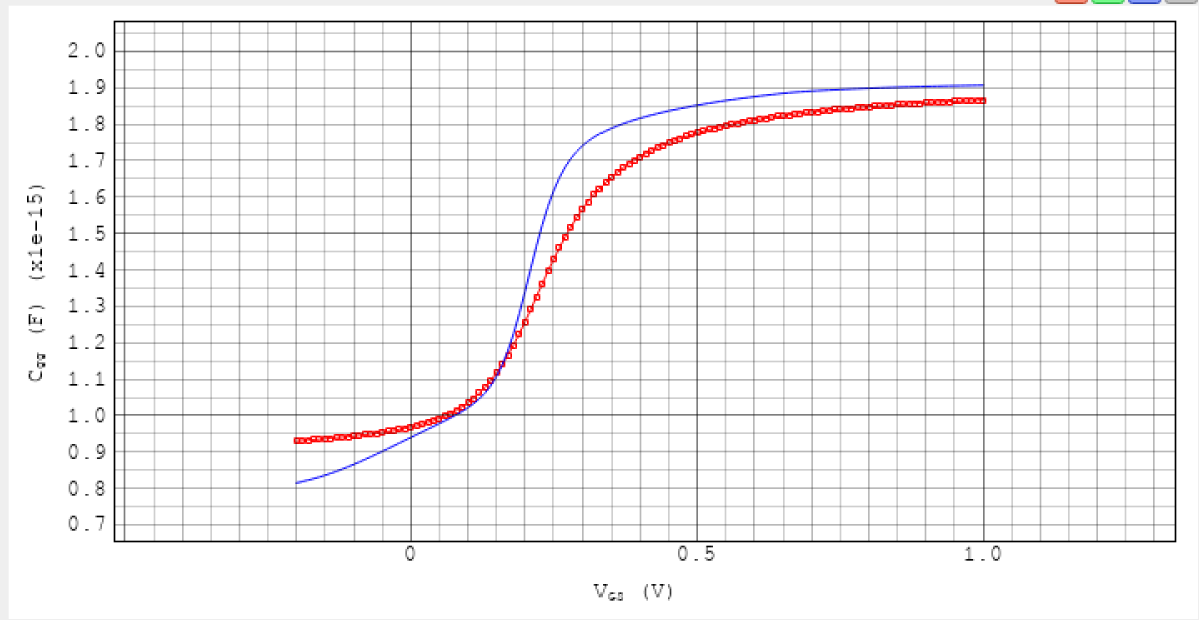
\includegraphics[width=0.9\textwidth]{image/task0.png}
	\caption{任务0结果：\(C_{gg}-V_{gs}\) 拟合}
\end{figure}

\section{任务1：阈值电压与亚阈值摆幅}

\subsection{原理分析}
阈值电压
\begin{equation}
	V_{th}=VTH0+K1\left(\sqrt{\Phi_s-V_{bs}}-\sqrt{\Phi_s}\right)-K2\,V_{bs}. \tag{BSIM4 (2.10)}
\end{equation}
亚阈值区漏电流
\begin{equation}
	I_{ds}=I_0\left[1-\exp\left(-\frac{V_{ds}}{v_t}\right)\right]\exp\left(\frac{V_{gs}-V_{th}-V'_{off}}{n v_t}\right). \tag{BSIM4 (3.19)}
\end{equation}
其中亚阈值摆幅参数 \(n\) 
\begin{equation}
	n=1+NFACTOR\frac{C_{dep}}{C_{oxe}}+\frac{Cdsc\text{-Term}+CIT}{C_{oxe}}. \tag{BSIM4 (3.21)}
\end{equation}
因此 \(CIT\) 会抬高 \(n\)，使 \(SS\) 变大（亚阈值斜率变缓）。

\subsection{调参过程与参数说明}
阈值提取时，实际操作采用固定电流法：
\begin{equation}
	I_{ref}=I_0\frac{W}{L},\qquad V_{th}=V_{gs}\ \text{at}\ I_{ds}=I_{ref}.
\end{equation}
本器件尺寸为 \(W=1\,\mu\mathrm{m}\)、\(L=65\,\mathrm{nm}\)，故
\begin{equation}
	\frac{W}{L}\approx 15.38.
\end{equation}
若取常见 \(I_0=100\,\mathrm{nA}\)，则
\begin{equation}
	I_{ref}\approx1.54\,\mu\mathrm{A}.
\end{equation}

本任务关键参数如下：
\begin{table}[H]
	\centering
	\caption{任务1关键参数}
	\begin{tabular}{@{}llll@{}}
		\toprule
		参数 & 本次值 & BSIM4 含义（单位） & 典型量级（手册默认） \\
		\midrule
		VTH0 & \(0.336002\,\mathrm{V}\) & 零体偏长沟道阈值电压（V） & 默认 \(0.7\,\mathrm{V}\)（NMOS） \\
		CIT & \(0.004034\,\mathrm{F/m^2}\) & 界面陷阱电容（F/m\(^2\)） & 常见为较小正值 \\
		\bottomrule
	\end{tabular}
\end{table}
\textbf{调参过程说明：} 
\begin{enumerate}
    \item 先调整 \(CIT\) 来拟合亚阈值区的斜率，使得 \(SS\) 与目标数据一致。
    \item 再调整 \(VTH0\) 来对齐 \(V_{th}\)，使得在 \(I_{ds}=I_{ref}\) 时 \(V_{gs}\) 与目标数据的 \(V_{th}\) 一致。
    \item 由于这一块受后续影响很多，所以确定 \(CIT\) 和 \(VTH0\) 后在后续调整过程中需要回头微调这两个参数来保持 \(V_{th}\) 和 \(SS\) 的对齐效果。但好在这两个参数主要影响亚阈值区，所以在调整过程中对它们的微调不会对其他区域的拟合效果造成太大影响，我们一般把他先调到大致拟合，在顺序靠后的过程中进行微调。
\end{enumerate}
\subsection{结果图展示与结论}
\begin{figure}[H]
	\centering
	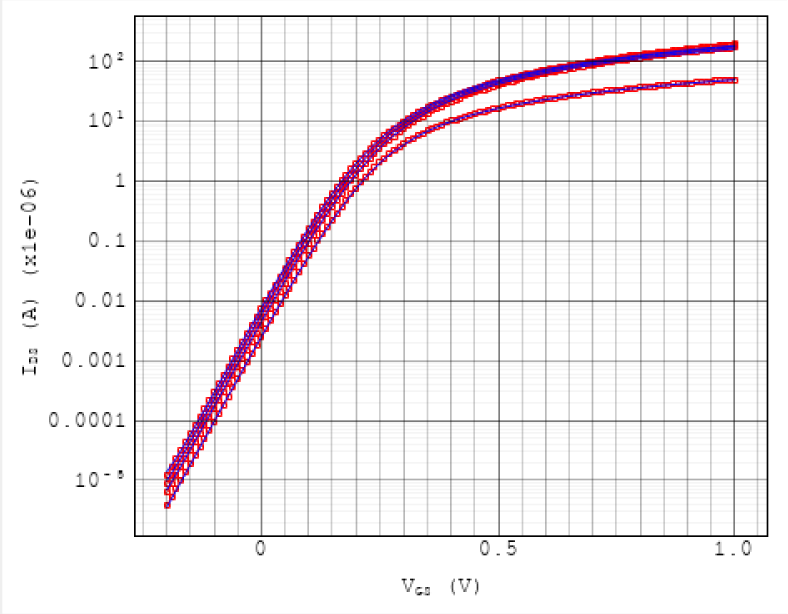
\includegraphics[width=0.78\textwidth]{image/task1.png}
	\caption{任务1总览：\(\log_{10}(I_{ds})-V_{gs}\) 拟合}
\end{figure}

\begin{figure}[H]
	\centering
	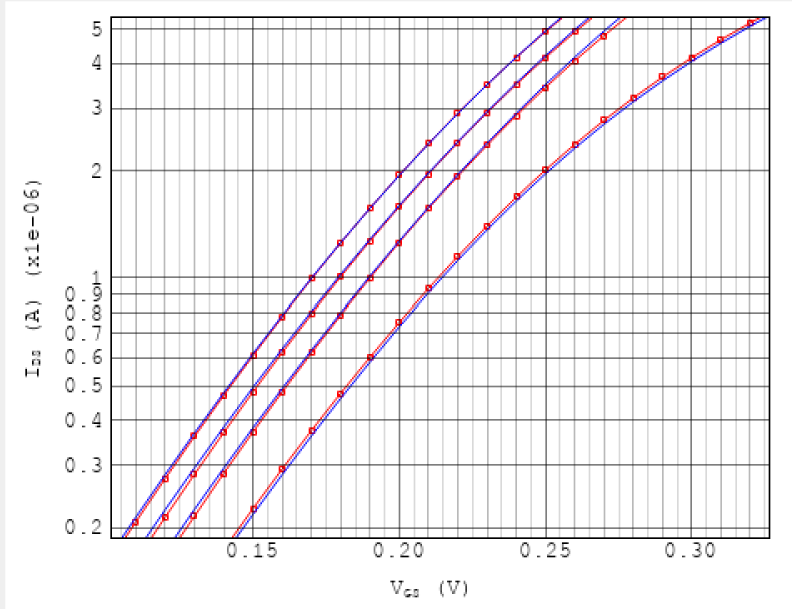
\includegraphics[width=0.78\textwidth]{image/task1_Vth.png}
	\caption{任务1局部：\(V_{th}\) 对齐}
\end{figure}

\begin{figure}[H]
	\centering
	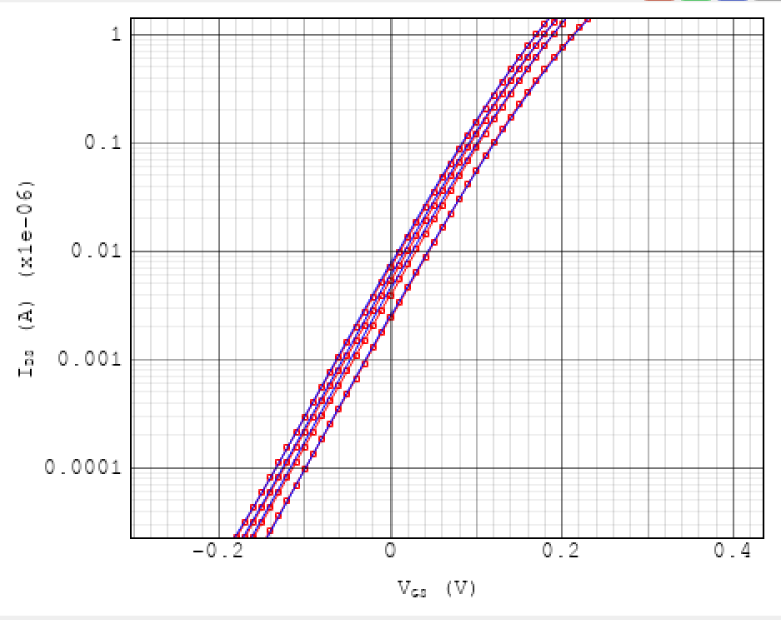
\includegraphics[width=0.78\textwidth]{image/task1_SS.png}
	\caption{任务1局部：\(SS\) 对齐}
\end{figure}

结果表明 \(VTH0\) 与 \(CIT\) 调整后，阈值偏移和亚阈值斜率拟合效果优秀。

\section{任务2：迁移率相关}

\subsection{原理分析}
本节使用 BSIM4 手册第5章 \(mobMod=2\) 的迁移率模型。手册式(5.8)为
\begin{equation}
	\mu_{eff}=\frac{U_0\,f(L_{eff})}{1+(UA+UC\cdot V_{bseff})\left[\frac{V_{gsteff}+C_0\cdot(VTH0-VFB-\Phi_s)}{TOXE}\right]^{EU}+UD\left(\frac{V_{th}\cdot TOXE}{V_{gsteff}+2\sqrt{V_{th}^2+0.0001}}\right)^2}. \tag{BSIM4 (5.8)}
\end{equation}
其中长度修正函数由式(5.9)给出
\begin{equation}
	f(L_{eff})=1-UP\cdot\exp\left(-\frac{L_{eff}}{LP}\right). \tag{BSIM4 (5.9)}
\end{equation}
同时，手册式(5.5)给出有效场近似
\begin{equation}
	E_{eff}\approx\frac{V_{gs}+V_{th}}{6TOXE}. \tag{BSIM4 (5.5)}
\end{equation}
由上式可知，\(U0\) 决定低场迁移率基值，\(UA\) 和 \(EU\) 决定高场退化与尾部斜率。

\paragraph{附：NDEP 对不同 \(V_{ds}\) 下 \(G_m\) 曲线间距的影响}
\(NDEP\) 不是直接写在迁移率式(5.8)中的参数，但它通过阈值模型耦合进 \(G_m\)：

\begin{equation}
\Phi_s = 0.4 + \frac{k_B T}{q}\ln\left(\frac{NDEP}{n_i}\right)+PHIN, \tag{BSIM4 (2.11)}
\end{equation}

\begin{equation}
\gamma_1 = \frac{\sqrt{2q\varepsilon_{si}NDEP}}{C_{oxe}}, \tag{BSIM4 (2.15)}
\end{equation}
\begin{equation}
V_{th}=VTH0+K1\left(\sqrt{\Phi_s-V_{bs}}-\sqrt{\Phi_s}\right)-K2V_{bs}. \tag{BSIM4 (2.10)}
\end{equation}

因此，当 \(U0\)、\(UA\)、\(EU\) 只能改变峰值高度/尾部斜率但难以改变不同 \(V_{ds}\) 曲线间距时，调整 \(NDEP\)（经 \(\Phi_s\)、\(K1\) 与 \(V_{th}\) 链路）会更有效地改变这种相对位置关系。

\subsection{调参过程与参数说明}
本任务关键参数如下：
\begin{table}[H]
	\centering
	\caption{任务2关键参数}
	\begin{tabular}{@{}llll@{}}
		\toprule
		参数 & 本次值 & BSIM4 含义（单位） & 典型量级（手册默认） \\
		\midrule
		U0 & \(0.0086\,\mathrm{m^2/(V\cdot s)}\) & 低场迁移率基值 & 默认 \(0.067\,\mathrm{m^2/(V\cdot s)}\)（NMOS） \\
		UA & \(1.5001\times10^{-10}\,\mathrm{m/V}\) & 一阶垂直场退化系数 & 常见 \(10^{-9}\sim10^{-15}\,\mathrm{m/V}\)\\
		EU & \(0.963833\) & \(mobMod=2\) 迁移率指数参数 & 默认 \(1.67\)（NMOS） \\
		\bottomrule
	\end{tabular}
\end{table}

\textbf{调参过程说明：}
\begin{enumerate}
    \item 首先调整 \(U0\) 来拟合低场区的 \(G_m\) 峰值。
    \item 再调整 \(UA\) 来修正高场区的 \(G_m\) 下降趋势。注意 \(UA\) 过大可能会导致过度退化，无法拟合目标数据。
    \item 最后微调 \(EU\) 来修正高场区尾部的斜率，使得整体曲线形状与目标数据一致。
    \item 由于 \(U0\) 的调整会影响 \(V_{th}\)，因此需要回到任务1重新微调 \(VTH0\) 来保持 \(V_{th}\) 的对齐。
    \item \(U0\) 和 \(UA\) 的调整效果会相互影响高场区的拟合效果，功能存在重叠，因此在调整过程中需协同改变\(U0\)和\(UA\)以达到最佳拟合效果。
    \item 由于 \(UA\) 和 \(EU\) 都影响高场区的退化行为，因此在调整时需要同时考虑两者的耦合关系。调参过程中发现\(EU\)从0到1过程中会极大影响\(UA\)的有效范围的数量级，所以在调整 \(EU\) 时需要重新评估 \(UA\) 的合理范围（从 \(10^{-11}\) 到 \(10^{-1}\)）。
    \item 调整过程中发现无论怎么调整\(U0\)，\(UA\) 和 \(EU\)都无法改变不同Vds下\(G_m\)曲线的相对位置关系（如增长速率之比），导致无法同时拟合低Vds和高Vds的\(G_m\)图线。经过尝试发现需要调整 \(NDEP\)来改变不同Vds下\(V_{th}\)的相对位置关系，在从（\(10^{27}\)到\(10^{22}\)取样尝试）才能同时拟合低Vds和高Vds的\(G_m\)峰值。
    \item 由于高\(V_gs\)下高\(V_ds\)不在考察重点，同时在尝试拟合该部分时发现需要协同调整V\(VSAT\)，\(U0\) 和 \(UA\)等参数，且这些参数会影响其他图线，我们在保证低\(V_ds\)下\(G_m\)峰值和整体趋势拟合效果的前提下，放弃对高\(V_ds\)下\(G_m\)峰值的拟合。
\end{enumerate}

\subsection{结果图展示与结论}
\begin{figure}[H]
	\centering
	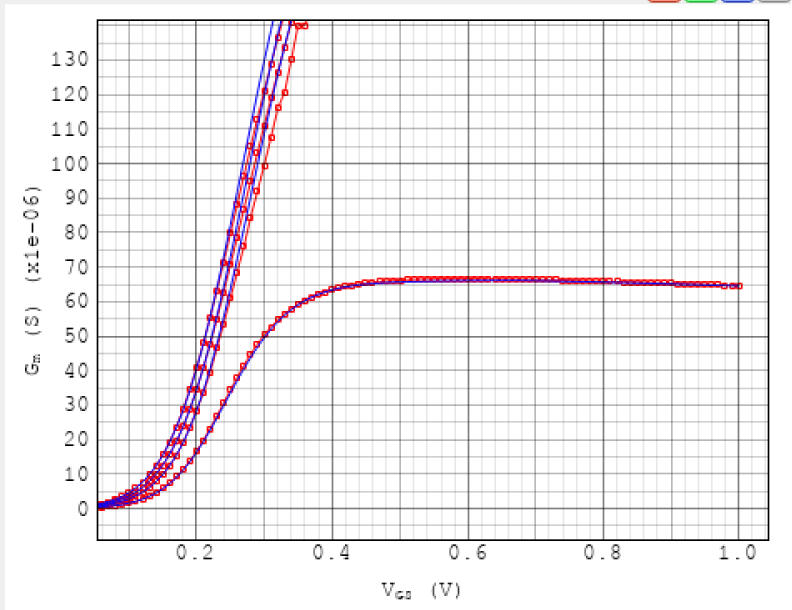
\includegraphics[width=0.78\textwidth]{image/task2_low_Vds.png}
	\caption{任务2局部（低 \(V_{ds}\)）：\(G_m-V_{gs}\) 拟合}
\end{figure}

\begin{figure}[H]
	\centering
	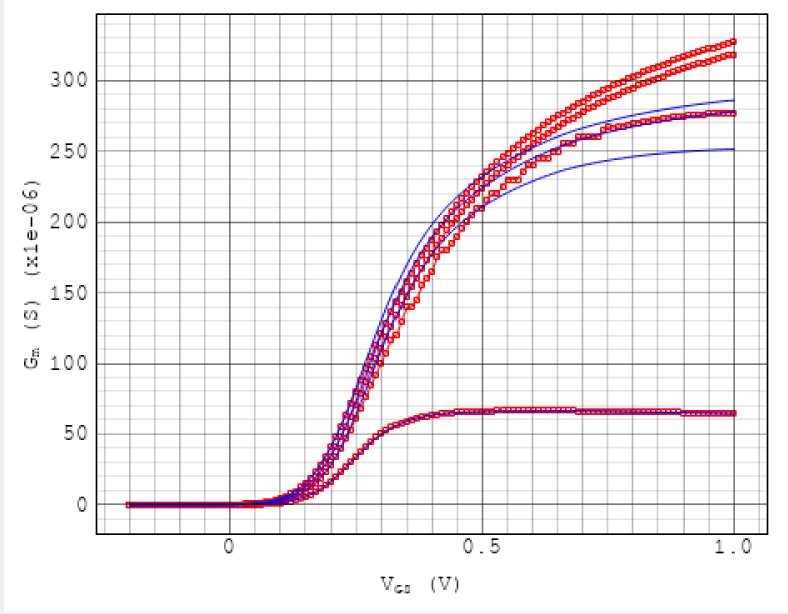
\includegraphics[width=0.78\textwidth]{image/task2.png}
	\caption{任务2总览：\(G_m-V_{gs}\) 拟合}
\end{figure}

结果显示在低 \(V_{ds}\) 条件下，\(G_m\) 图线拟合优秀。

\section{任务3：漏致势垒降低（DIBL）}
\vspace{7cm}

\section{任务4：饱和速度、沟长调制与过渡平滑}
\vspace{7cm}

\section{任务5：进一步调整}
\vspace{7cm}

\end{document}
